\section{Multivariate ANOVA}
\frame{\sectionpage}


\begin{frame}[fragile]{Multivariate analysis of variance}

  \begin{itemize}
  \item Standard ANOVA has just one response variable.
  \item What if you have more than one response?
  \item Try an ANOVA on each response separately.
  \item But might miss some kinds of interesting dependence between the responses that distinguish the groups.
  \end{itemize}
  
\end{frame}

\begin{frame}[fragile]{Small example}

  \begin{itemize}
  \item Measure yield and seed weight of plants grown under 2 conditions: low and high amounts of fertilizer.
  \item Data (fertilizer, yield, seed weight):


 
\begin{knitrout}
\definecolor{shadecolor}{rgb}{0.969, 0.969, 0.969}\color{fgcolor}\begin{kframe}
\begin{alltt}
\hlstd{hilo}\hlkwb{=}\hlkwd{read.table}\hlstd{(}\hlstr{"manova1.txt"}\hlstd{,}\hlkwc{header}\hlstd{=T)}
\hlstd{hilo}
\end{alltt}
\begin{verbatim}
##   fertilizer yield weight
## 1        low    34     10
## 2        low    29     14
## 3        low    35     11
## 4        low    32     13
## 5       high    33     14
## 6       high    38     12
## 7       high    34     13
## 8       high    35     14
\end{verbatim}
\end{kframe}
\end{knitrout}

  \item 2 responses, yield and seed weight.
  \end{itemize}
  
\end{frame}

\begin{frame}[fragile]{Boxplot for yield for each fertilizer group}

 
\begin{knitrout}
\definecolor{shadecolor}{rgb}{0.969, 0.969, 0.969}\color{fgcolor}\begin{kframe}
\begin{alltt}
\hlkwd{ggplot}\hlstd{(hilo,}\hlkwd{aes}\hlstd{(}\hlkwc{x}\hlstd{=fertilizer,}\hlkwc{y}\hlstd{=yield))}\hlopt{+}\hlkwd{geom_boxplot}\hlstd{()}
\end{alltt}
\end{kframe}
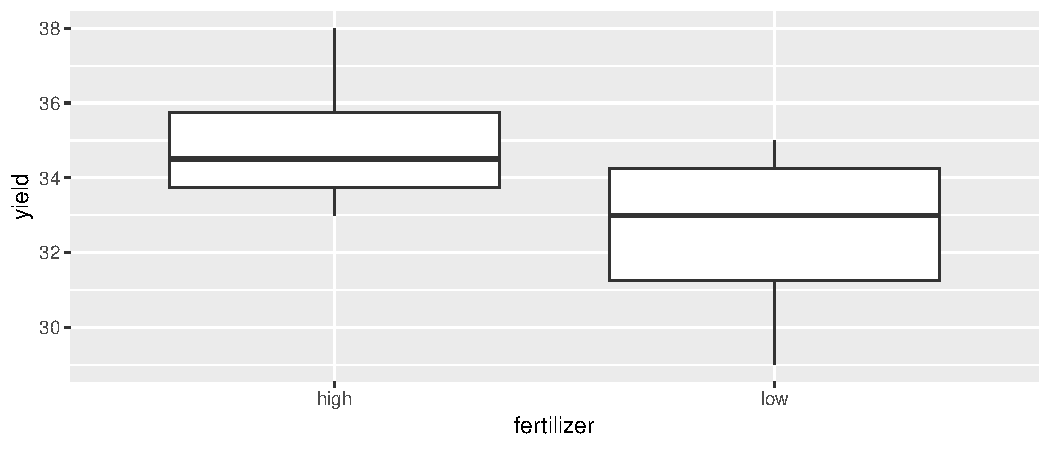
\includegraphics[width=\maxwidth]{figure/ferto-1} 

\end{knitrout}
  
  

Yields overlap for fertilizer groups.
  
\end{frame}

\begin{frame}[fragile]{Boxplot for weight for each fertilizer group}

 
\begin{knitrout}
\definecolor{shadecolor}{rgb}{0.969, 0.969, 0.969}\color{fgcolor}\begin{kframe}
\begin{alltt}
\hlkwd{ggplot}\hlstd{(hilo,}\hlkwd{aes}\hlstd{(}\hlkwc{x}\hlstd{=fertilizer,}\hlkwc{y}\hlstd{=weight))}\hlopt{+}\hlkwd{geom_boxplot}\hlstd{()}
\end{alltt}
\end{kframe}
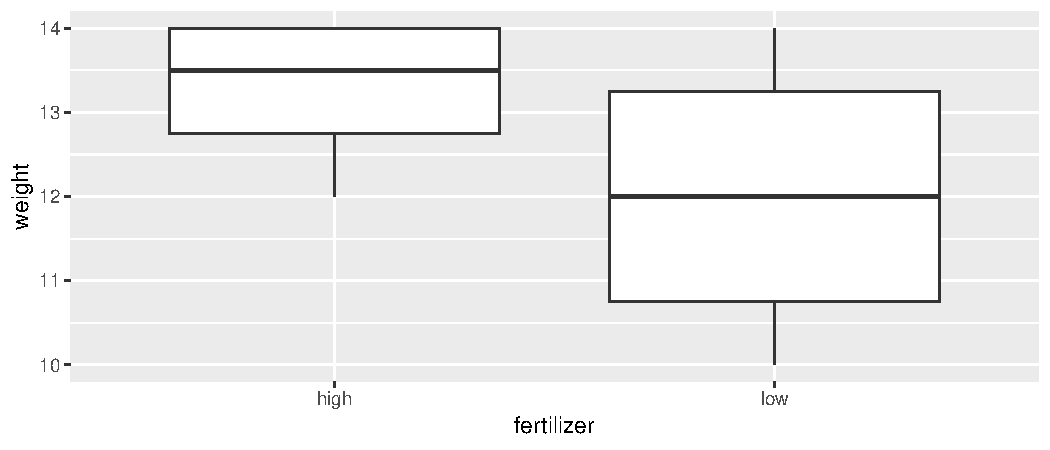
\includegraphics[width=\maxwidth]{figure/casteldisangro-1} 

\end{knitrout}

Weights overlap for fertilizer groups.
  
\end{frame}

\begin{frame}[fragile]{ANOVAs for yield and weight}

{\small
 
\begin{knitrout}
\definecolor{shadecolor}{rgb}{0.969, 0.969, 0.969}\color{fgcolor}\begin{kframe}
\begin{alltt}
\hlstd{hilo.y}\hlkwb{=}\hlkwd{aov}\hlstd{(yield}\hlopt{~}\hlstd{fertilizer,}\hlkwc{data}\hlstd{=hilo)}
\hlkwd{summary}\hlstd{(hilo.y)}
\end{alltt}
\begin{verbatim}
##             Df Sum Sq Mean Sq F value Pr(>F)
## fertilizer   1   12.5  12.500   2.143  0.194
## Residuals    6   35.0   5.833
\end{verbatim}
\begin{alltt}
\hlstd{hilo.w}\hlkwb{=}\hlkwd{aov}\hlstd{(weight}\hlopt{~}\hlstd{fertilizer,}\hlkwc{data}\hlstd{=hilo)}
\hlkwd{summary}\hlstd{(hilo.w)}
\end{alltt}
\begin{verbatim}
##             Df Sum Sq Mean Sq F value Pr(>F)
## fertilizer   1  3.125   3.125   1.471  0.271
## Residuals    6 12.750   2.125
\end{verbatim}
\end{kframe}
\end{knitrout}
}

Neither response depends significantly on fertilizer. But\ldots
  
\end{frame}

\begin{frame}[fragile]{Plotting both responses at once}

Have two response variables (not more), so can plot the
response variables against \emph{each other}, labelling points by
which fertilizer group they're from.

\begin{knitrout}
\definecolor{shadecolor}{rgb}{0.969, 0.969, 0.969}\color{fgcolor}\begin{kframe}
\begin{alltt}
\hlstd{g}\hlkwb{=}\hlkwd{ggplot}\hlstd{(hilo,}\hlkwd{aes}\hlstd{(}\hlkwc{x}\hlstd{=yield,}\hlkwc{y}\hlstd{=weight,}\hlkwc{colour}\hlstd{=fertilizer))}\hlopt{+}
  \hlkwd{geom_point}\hlstd{()}
\end{alltt}
\end{kframe}
\end{knitrout}

Also want line through
points $(31,14)$ and $(38,10)$ (see why later):

\begin{knitrout}
\definecolor{shadecolor}{rgb}{0.969, 0.969, 0.969}\color{fgcolor}\begin{kframe}
\begin{alltt}
\hlstd{line_x}\hlkwb{=}\hlkwd{c}\hlstd{(}\hlnum{31}\hlstd{,}\hlnum{38}\hlstd{)}
\hlstd{line_y}\hlkwb{=}\hlkwd{c}\hlstd{(}\hlnum{14}\hlstd{,}\hlnum{10}\hlstd{)}
\hlstd{d}\hlkwb{=}\hlkwd{data.frame}\hlstd{(line_x,line_y)}
\hlstd{g}\hlkwb{=}\hlstd{g}\hlopt{+}\hlkwd{geom_smooth}\hlstd{(}\hlkwc{data}\hlstd{=d,}\hlkwd{aes}\hlstd{(}\hlkwc{x}\hlstd{=line_x,}\hlkwc{y}\hlstd{=line_y,}\hlkwc{colour}\hlstd{=}\hlkwa{NULL}\hlstd{),}
  \hlkwc{method}\hlstd{=}\hlstr{"lm"}\hlstd{,}\hlkwc{se}\hlstd{=F)}
\end{alltt}
\end{kframe}
\end{knitrout}

I am fitting a regression line through the points in \texttt{d}. I am
adding to a previous \texttt{ggplot}, so my \texttt{geom\_smooth} is
inheriting the \texttt{colour} from the first one. This data frame has
no \texttt{fertilizer} (what previous \texttt{colour} was), so I have to unset it.
  
\end{frame}

\begin{frame}[fragile]{The plot}
  
 
\begin{knitrout}
\definecolor{shadecolor}{rgb}{0.969, 0.969, 0.969}\color{fgcolor}\begin{kframe}
\begin{alltt}
\hlstd{g}
\end{alltt}
\end{kframe}
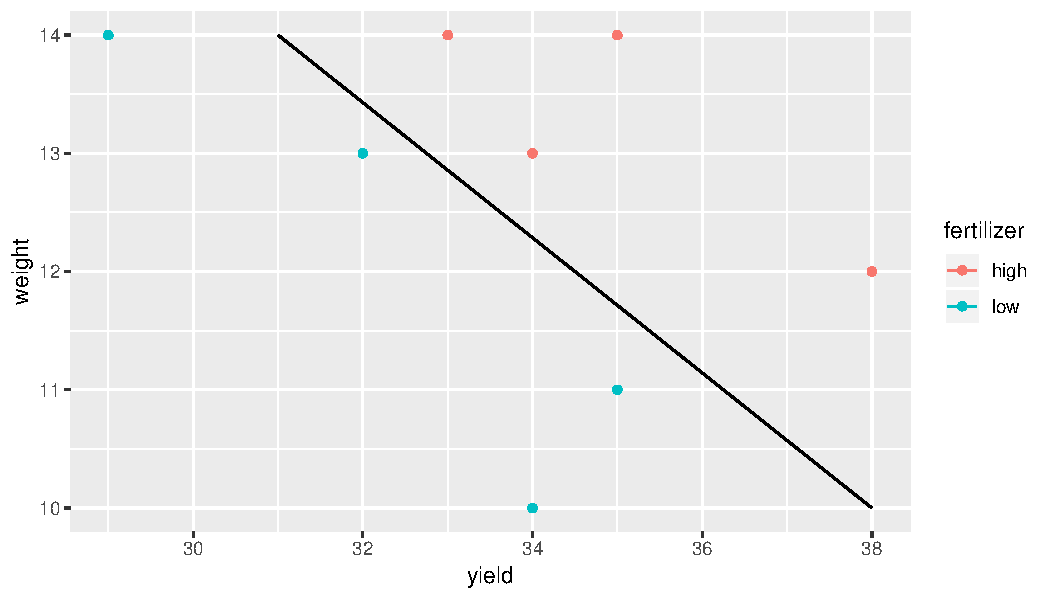
\includegraphics[width=\maxwidth]{figure/charlecombe-1} 

\end{knitrout}
  
  
\end{frame}

\begin{frame}[fragile]{MANOVA}
  
\begin{knitrout}
\definecolor{shadecolor}{rgb}{0.969, 0.969, 0.969}\color{fgcolor}\begin{kframe}
\begin{alltt}
\hlstd{g}
\end{alltt}
\end{kframe}
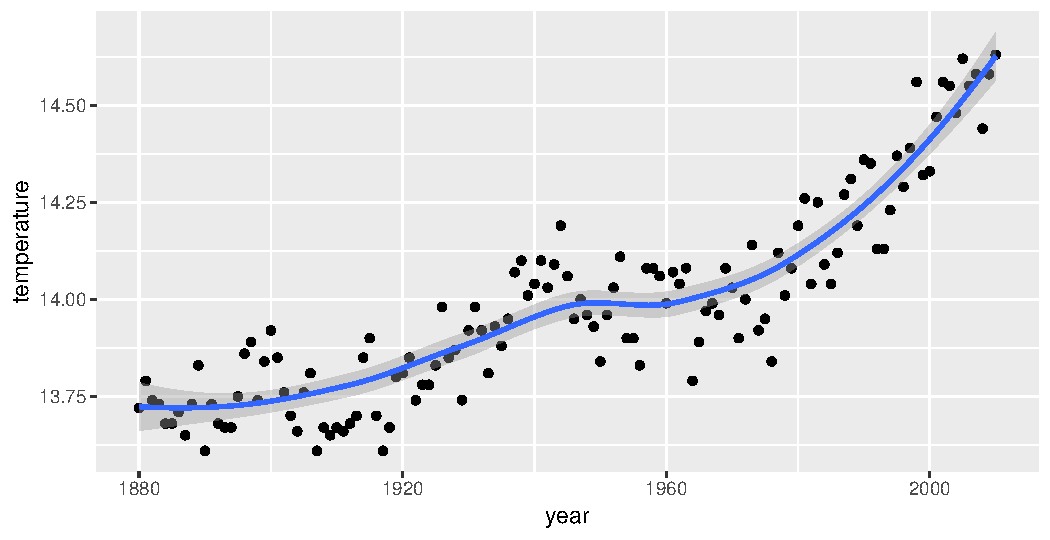
\includegraphics[width=\maxwidth]{figure/unnamed-chunk-6-1} 

\end{knitrout}
  \begin{itemize}
  \item High-fertilizer plants have both yield and weight high.
  \item True even though no sig difference in yield or weight individually.
  \item Drew line separating highs from lows on plot.
  \end{itemize}

 

\end{frame}

\begin{frame}[fragile]{MANOVA finds multivariate differences}
  
  \begin{itemize}
  \item Is difference found by diagonal line significant? MANOVA finds out.

  \end{itemize}

  \begin{small}
\begin{knitrout}
\definecolor{shadecolor}{rgb}{0.969, 0.969, 0.969}\color{fgcolor}\begin{kframe}
\begin{alltt}
\hlstd{response}\hlkwb{=}\hlkwd{with}\hlstd{(hilo,}\hlkwd{cbind}\hlstd{(yield,weight))}
\hlstd{hilo.1}\hlkwb{=}\hlkwd{manova}\hlstd{(response}\hlopt{~}\hlstd{fertilizer,}\hlkwc{data}\hlstd{=hilo)}
\hlkwd{summary}\hlstd{(hilo.1)}
\end{alltt}
\begin{verbatim}
##            Df  Pillai approx F num Df den Df  Pr(>F)  
## fertilizer  1 0.80154   10.097      2      5 0.01755 *
## Residuals   6                                         
## ---
## Signif. codes:  0 '***' 0.001 '**' 0.01 '*' 0.05 '.' 0.1 ' ' 1
\end{verbatim}
\end{kframe}
\end{knitrout}
    
  \end{small}

Yes! Difference between groups is \emph{diagonally}, not just up/down
(weight) or left-right (yield). The \emph{yield-weight combination} matters.
  
\end{frame}

\begin{frame}[fragile]{Strategy}

\begin{itemize}
\item Create new response variable by gluing together columns of
  responses, using \texttt{cbind}.
\item Use \texttt{manova} with new response, looks like \texttt{lm} otherwise.
\item With more than 2 responses, cannot draw graph. What then?
\item If MANOVA test significant, cannot use Tukey. What then?
\item Use {\em discriminant analysis} (of which more later).
\end{itemize}

\end{frame}

\begin{frame}[fragile]{Another way to do MANOVA}

  
  \begin{itemize}
  \item Install package \texttt{car}, then:
  
{\small
 
\begin{knitrout}
\definecolor{shadecolor}{rgb}{0.969, 0.969, 0.969}\color{fgcolor}\begin{kframe}
\begin{alltt}
\hlstd{hilo.2.lm}\hlkwb{=}\hlkwd{lm}\hlstd{(response}\hlopt{~}\hlstd{fertilizer,}\hlkwc{data}\hlstd{=hilo)}
\hlstd{hilo.2}\hlkwb{=}\hlstd{car}\hlopt{::}\hlkwd{Manova}\hlstd{(hilo.2.lm)}
\hlstd{hilo.2}
\end{alltt}
\begin{verbatim}
## 
## Type II MANOVA Tests: Pillai test statistic
##            Df test stat approx F num Df den Df  Pr(>F)  
## fertilizer  1   0.80154   10.097      2      5 0.01755 *
## ---
## Signif. codes:  0 '***' 0.001 '**' 0.01 '*' 0.05 '.' 0.1 ' ' 1
\end{verbatim}
\end{kframe}
\end{knitrout}

}

  
\item Or \texttt{library(car)} followed by \texttt{Manova(...)}.
\item Same result as small-m \texttt{manova}.
\item \texttt{Manova} will also do \emph{repeated measures}, coming up.
\end{itemize}
  
\end{frame}

\begin{frame}[fragile]{Another example: peanuts}

  \begin{itemize}
  \item  Three different varieties
of peanuts (mysteriously, 5, 6 and 8) planted in two different
locations.
\item Three response variables: \texttt{y}, \texttt{smk} and
\texttt{w}.
  \end{itemize}

 
\begin{knitrout}
\definecolor{shadecolor}{rgb}{0.969, 0.969, 0.969}\color{fgcolor}\begin{kframe}
\begin{alltt}
\hlstd{peanuts.orig}\hlkwb{=}\hlkwd{read.table}\hlstd{(}\hlstr{"peanuts.txt"}\hlstd{,}\hlkwc{header}\hlstd{=T)}
\hlkwd{head}\hlstd{(peanuts.orig)}
\end{alltt}
\begin{verbatim}
##   obs location variety     y   smk    w
## 1   1        1       5 195.3 153.1 51.4
## 2   2        1       5 194.3 167.7 53.7
## 3   3        2       5 189.7 139.5 55.5
## 4   4        2       5 180.4 121.1 44.4
## 5   5        1       6 203.0 156.8 49.8
## 6   6        1       6 195.9 166.0 45.8
\end{verbatim}
\end{kframe}
\end{knitrout}
    
    
\end{frame}

\begin{frame}[fragile]{Setup for analysis}

  Using \texttt{dplyr}:
 
\begin{knitrout}
\definecolor{shadecolor}{rgb}{0.969, 0.969, 0.969}\color{fgcolor}\begin{kframe}
\begin{alltt}
\hlstd{peanuts.orig} \hlopt
  \hlkwd{mutate}\hlstd{(}\hlkwc{location}\hlstd{=}\hlkwd{factor}\hlstd{(location),}
         \hlkwc{variety}\hlstd{=}\hlkwd{factor}\hlstd{(variety))} \hlkwb{->} \hlstd{peanuts}
\hlstd{response}\hlkwb{=}\hlkwd{with}\hlstd{(peanuts,}\hlkwd{cbind}\hlstd{(y,smk,w))}
\hlkwd{head}\hlstd{(response)}
\end{alltt}
\begin{verbatim}
##          y   smk    w
## [1,] 195.3 153.1 51.4
## [2,] 194.3 167.7 53.7
## [3,] 189.7 139.5 55.5
## [4,] 180.4 121.1 44.4
## [5,] 203.0 156.8 49.8
## [6,] 195.9 166.0 45.8
\end{verbatim}
\end{kframe}
\end{knitrout}

  
\end{frame}

\begin{frame}[fragile]{Analysis (using \texttt{Manova})}

{\footnotesize  
 
\begin{knitrout}
\definecolor{shadecolor}{rgb}{0.969, 0.969, 0.969}\color{fgcolor}\begin{kframe}
\begin{alltt}
\hlstd{peanuts.1}\hlkwb{=}\hlkwd{lm}\hlstd{(response}\hlopt{~}\hlstd{location}\hlopt{*}\hlstd{variety,}\hlkwc{data}\hlstd{=peanuts)}
\hlstd{peanuts.2}\hlkwb{=}\hlstd{car}\hlopt{::}\hlkwd{Manova}\hlstd{(peanuts.1)}
\hlstd{peanuts.2}
\end{alltt}
\begin{verbatim}
## 
## Type II MANOVA Tests: Pillai test statistic
##                  Df test stat approx F num Df den Df   Pr(>F)   
## location          1   0.89348  11.1843      3      4 0.020502 * 
## variety           2   1.70911   9.7924      6     10 0.001056 **
## location:variety  2   1.29086   3.0339      6     10 0.058708 . 
## ---
## Signif. codes:  0 '***' 0.001 '**' 0.01 '*' 0.05 '.' 0.1 ' ' 1
\end{verbatim}
\end{kframe}
\end{knitrout}
}  

\begin{itemize}
\item Interaction not quite significant, but main effects are.
\item Combined response variable \texttt{(y,smk,w)} definitely depends
  on location and on variety
\item Weak dependence of \texttt{(y,smk,w)} on the location-variety \emph{combination.}
\item Understanding that dependence beyond our scope right now.
\end{itemize}

  
\end{frame}
